%-------------------------------------------------------------------------------
\section{Introduction}
\label{s:intro}
%-------------------------------------------------------------------------------

Many microservices contend with varying load as well as being \textit{latency
critical} (LC), meaning they have strict SLOs that guarantee uptime and caps on
latency. However, when developers want to run microservices, scheduling systems
like AWS ec2 or Kubernetes require them to give a fixed amount of resources the
microservice needs, \ie{} a number of CPUs and an amount of
memory~\cite{aws-ec2-resources, kubernetes-resources}. As a result, developers
choose those requirements based on the expected peak load, and the resources are
rarely fully used~\cite{borg, nu, overprovision}.

Other tasks do not fall into this category: \textit{best effort} (BE) tasks such
as long-running map reduce jobs or background data analytics do not have an SLO.

Indeed, many modern scheduling systems separate the work they run into classes,
that include one class for LC tasks, which have resource requirements, and one
class for BE tasks, which don't. This includes distributed schedulers, \eg{}
Borg\cite{borg} or Kubernetes\cite{kubernetes-resources}, and single machine
schedulers, \eg{} Caladan\cite{caladan}.

In an ideal world, BE tasks allows providers to get high utilization by
oversubscribing their machines without compromising any guarantees: Under high
load, microservice workloads run without impediment, but in low load BE tasks
run opportunistically and the servers maintain high utilization.

However, realizing high utilization while enforcing strict isolation is
challenging. The scheduler needs to dynamically reallocate CPUs as the load
changes: it needs to maintain low latencies for LC requests by ensuring that
when the LC processes need resources they appear uncontended, while at the same
time using idle resources to run BE processes.

\begin{figure}[t]
    \centering
    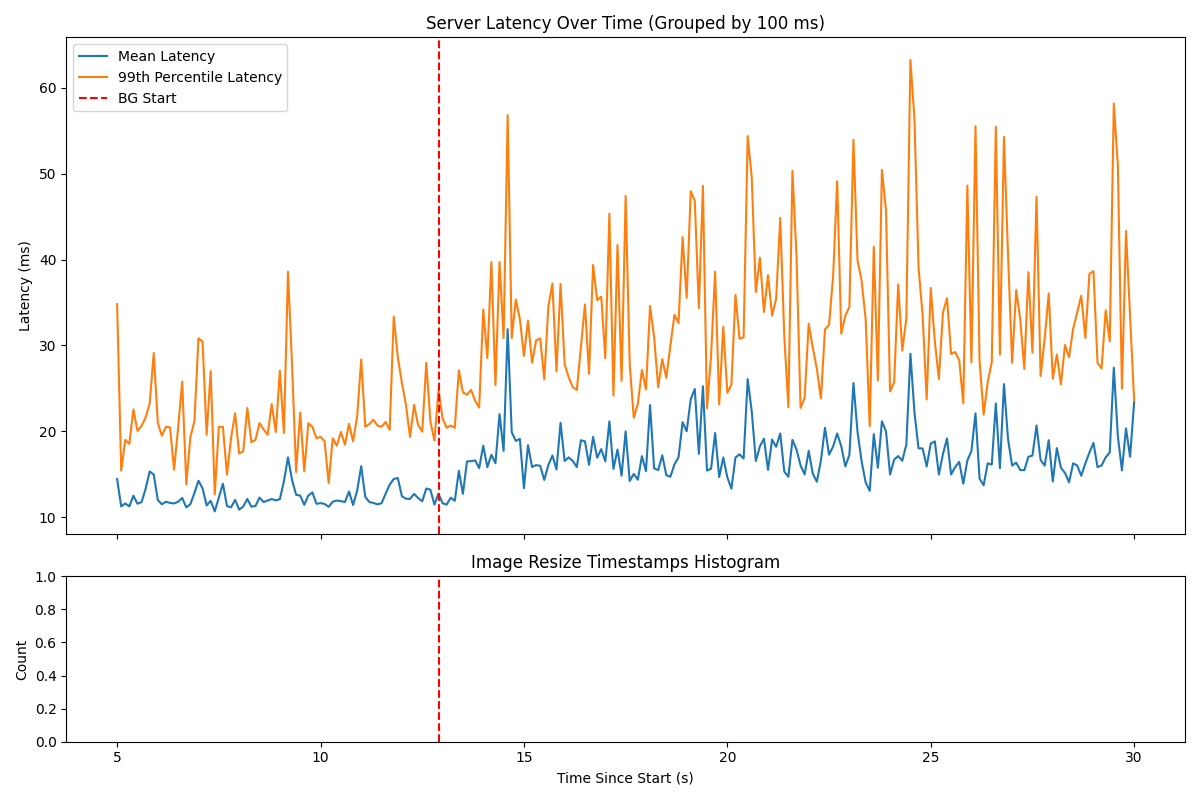
\includegraphics[width=\columnwidth]{graphs/kubernetes-unedited.png}
    \caption{E2E repsonse times for a simple social network web application,
    before and after starting load on a BE
    service}\label{fig:kubernetes-unedited}
\end{figure}

Current popular systems fail to properly isolate latency critical from best
effort workloads. When running a small but realistic social network web
application on Kubernetes, we observe significant impacts on its latency when
starting a best effort workload, doing image resizing, on the same machine.
\autoref{fig:kubernetes-unedited} plots the end-to-end latency of an endpoint
that gets a users feed on the top graph; the bottom graph shows the throughput
of the BE workload. The mean response latency jumps from $\sim$7ms to
$\sim$15ms, and the 99th percentile latency from $\sim$10ms to $\sim$23ms. 

Understanding where the isolation fails requires understanding the underlying
mechanism that is enforcing the cpu isolation: The current standard mechanism
for isolating LC from BE processes is Linux's \cgroups{}.\hmng{I kinda snuck in
the jump from "isolation" to "cpu isolation". Probably should at some point just
state and then move on that we focus on cpu} Most modern containers rely on
\cgroups{}; this includes all Open Container Initiative (OCI) compliant
containers, including Kubernetes but also Docker, CRI-O, and
containerd~\cite{oci-cgroups,docker-docs-cgroups,container-isolation-article}.
VMs, including Firecracker, AFaas, and KVM, also rely on \cgroups{} to manage
CPU time allocation when the number of vCPUs is
oversubscribed.~\cite{kvm-cgroups, firecracker-cgroups,afaas}

The part of the \cgroups{} interface that these systems use to specify the
priority of processes is based on weight: each workload is put into its own
group, and each group is assigned a weight in the range [1, 10000]. \cgroups{}
specifies that each group gets CPU time proportional to its weight as a share of
the sum of weights of runnable groups~\cite{cgroups-kerneldocs}.\footnote{Other
operating systems use a similar interface, for instance Windows exposes a number
of shares.} For instance, if two groups $cg1$ and $cg2$ have weights 200 and 300
respectively, when they are both active their CPU time ratio should also be
$2:3$. However, if $cg1$ has no runnable threads, then $cg2$ would represent
100\% of the runnable weight and get all the CPU time.

\begin{figure}[t]
    \centering
    \begin{subfigure}[b]{0.49\columnwidth}
        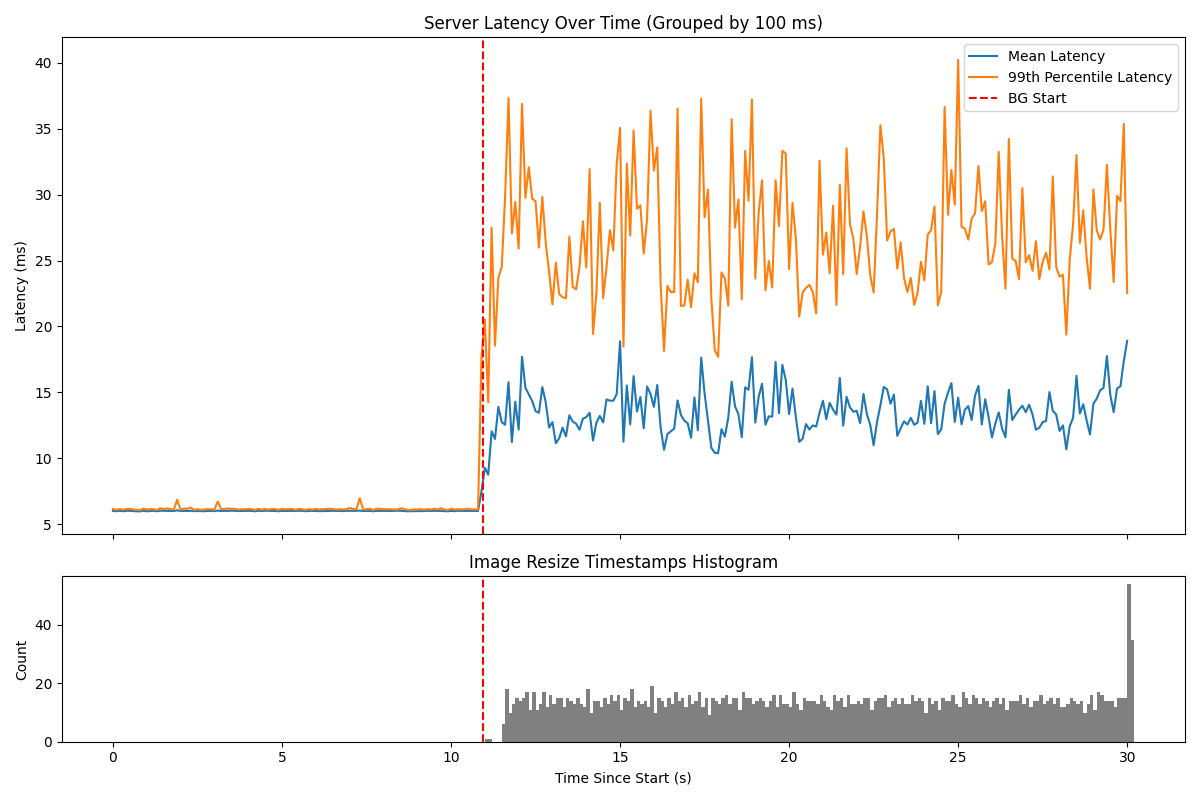
\includegraphics[width=\columnwidth]{graphs/srv-bg-unedited-low.png}
        \caption{Low load stetting, utilization before starting the BE tasks is
        around 85\%}\label{fig:srv-bg-unedited-low}
    \end{subfigure}
    \hspace{\fill}
    \begin{subfigure}[b]{0.49\columnwidth}
        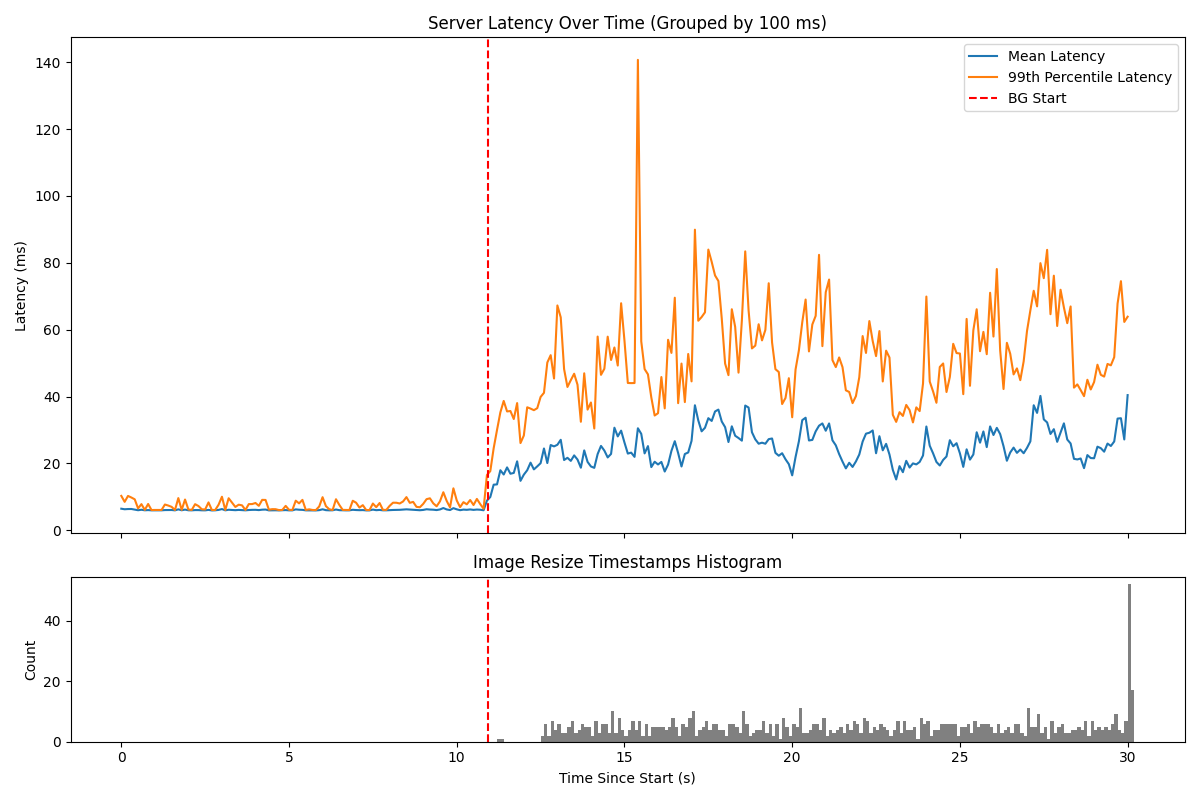
\includegraphics[width=\columnwidth]{graphs/srv-bg-unedited-high.png}
        \caption{High load setting, utilization before starting the BE tasks is
        around 95\%}\label{fig:srv-bg-unedited-high}
    \end{subfigure}
    \vspace{4pt}
    \caption{Latencies of the server and iteration counts of the background
    tasks in different load scenarios. Note the different y axis limits. The
    upper graphs show end-to-end request latencies, and the bottom graph is a
    histogram of completed iterations of the BE tasks}\label{fig:srv-bg-unedited}
\end{figure}

We reproduce the jump in latency we saw in the application running on Kubernetes
in a simpler benchmark. We run a simple cpu-bound server and then start two BE
workloads doing image resizing, using two \cgroups{} groups, with weights 1 and
10000, to isolate the two. \autoref{fig:srv-bg-unedited} shows the increase in
latencies of the LC server at two different baseline utilization levels. We see
that even in the lower baseline utilization case, where the server alone uses
85\%, mean latencies spike up from steady at around 6ms to as high as 20ms, and
much higher for 99th percentile latencies.

This shows that the failure to isolate LC workloads from BE ones will show up in
any system that uses \cgroups{}, which includes basically all the most popular
containers and VMs.

As we explore in \autoref{s:problem}, the main place \cgroups{} isolation fails
is that Linux allows BE processes to run on one core, even while another core
has a queued and waiting LC process. This is an interface problem, not an
implementation bug: Linux's scheduler uses per-core runqueues, and as a result
the weights are only enforced on a runqeueue level.

This paper argues that the split between LC and BE should be categorical rather
than ends of a weight spectrum, and that unfairness should be the goal. We show
that doing so enables Linux to isolate LC from BE:\ in the same experiment, the
increase in average latency when starting a BE workload goes from $>$2x to 0,
and the tail latency from $>$5x to 0. The contributions of this paper are thus
as follows: \hmng{given this new intro flow the contributions feel a bit too
Linux-specific?}
\begin{enumerate}
    \item the insight that weighted fair share breaks down with large weight
    splits because the weights are not enforced across cores; and that this
    dramatically affects end-to-end latencies
    \item showing that categorical priorities are simpler to enforce, and that
    Linux does this well
    \item implement in Linux \schedbe{}, a new class for BE tasks that is
    categorically separate from the default class LC tasks run in, which
    isolates LC workloads from BE ones and minimizes the amount of cross-core
    checks required
\end{enumerate}
